\section{Computational Rationality}

Comp. Rationality converges ideas from AI, robotics, cognitive science and neurosciences. 

It refers to computational principles for:
\begin{enumerate}[itemsep=-5pt, topsep=-20pt, leftmargin=*]
    \item Identifying decisions with highest expected utility, while taking into consideration the costs of computation in complex real-world problem, where calculations can only be approximated.
    \item Implementing bounded optimality in humans. 
\end{enumerate}

\textbf{Why User Models}

\begin{itemize}[itemsep=-5pt, topsep=-20pt, leftmargin=*]
	\item Used as test to help in creation and validation of new HCI theories
	\item Helps design more robust interaction, with improved safety and accessibility
	\item Reduce financial, temporal and human costs of usability testing
	\item Helps take advantage of advances in other engineering disciplines
	\item Advance next generation of intelligent interactive systems
\end{itemize}

\textit{Limitations to Model human processor} \smallskip

\begin{itemize}[itemsep=-5pt, topsep=-20pt, leftmargin=*]
	\item does not learn, adapt, generalize and has othe tradeoffs
\end{itemize}
Interaction is not equal to emerging behavior. After initial task has failed/succeded, there is no adaptive behavior or reorganization without explicit instruction.

\textit{Complexities of real-world tasks} \smallskip

\begin{itemize}[itemsep=-5pt, topsep=-20pt, leftmargin=*]
	\item Generalization: Go from precious episodes to an unseen one
	\item Latent learning: Adapting to distal changes in environment
	\item Planning: Sequencing actions while considering long-term effects on reward
	\item Compositionality: Good solution require putting together partial solutions cleverly
	\item Exploration/exploitation: Knowing when to learn the structure of task /environment vs when to exploit it
	\item Uncertainty: Knowledge can be incomplete or incorrect
	\item Resource limitations: Limited time and capabilities
	\item Curse of dimensionality: A very large number of possibilities
\end{itemize}

\begin{center}
	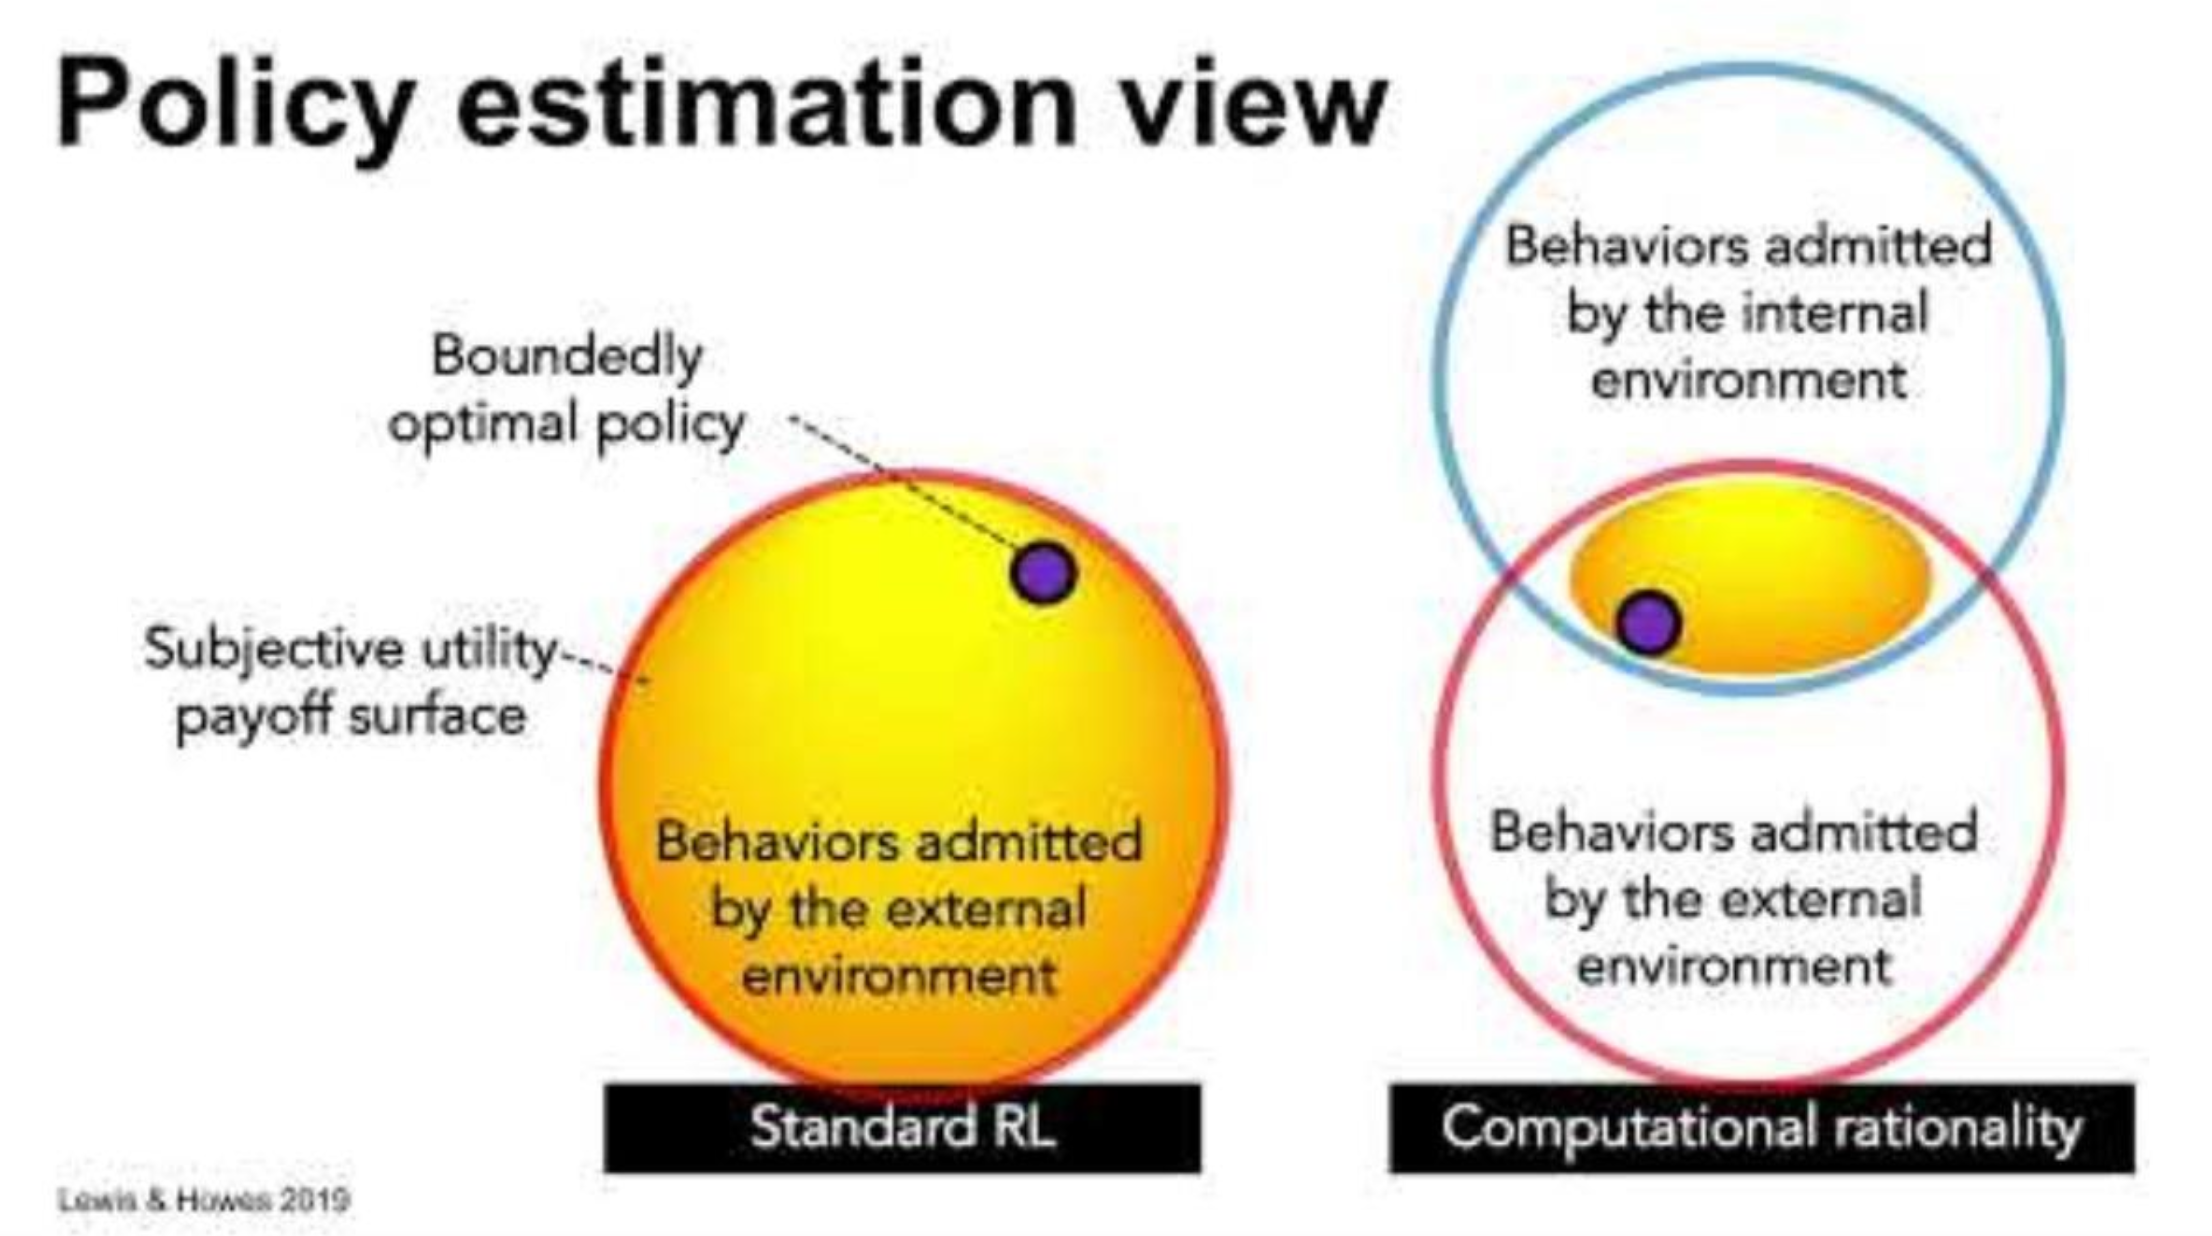
\includegraphics[width=\linewidth]{policy_estimation_view.png}
\end{center}


\textbf{Optimal Policy}

Is supposed to look at emerging bahavior component. \medskip

\textit{Interactions as a sequential decision-making process} \smallskip

\begin{center}
	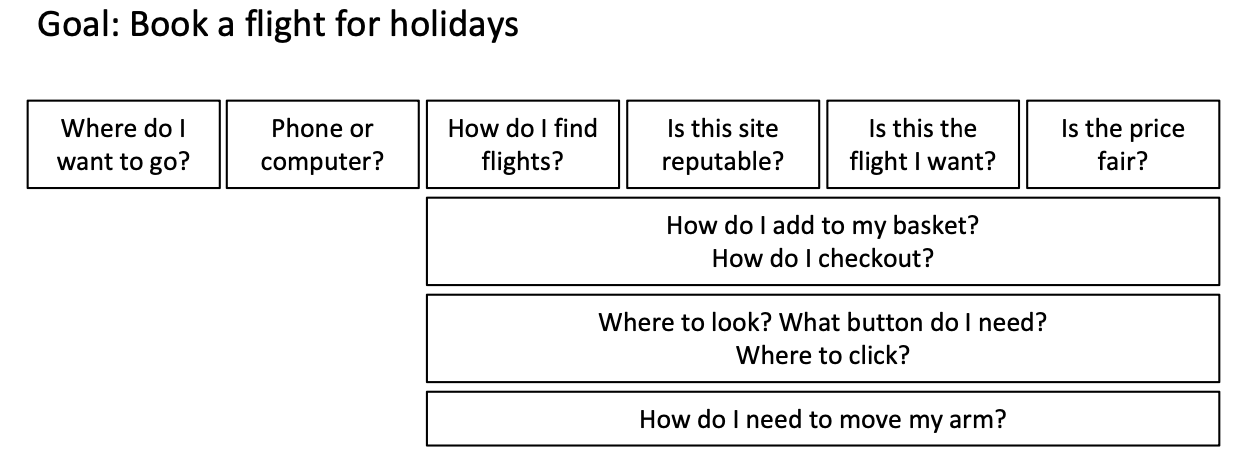
\includegraphics[width=\linewidth]{book_flights.png}
\end{center}

\begin{center}
	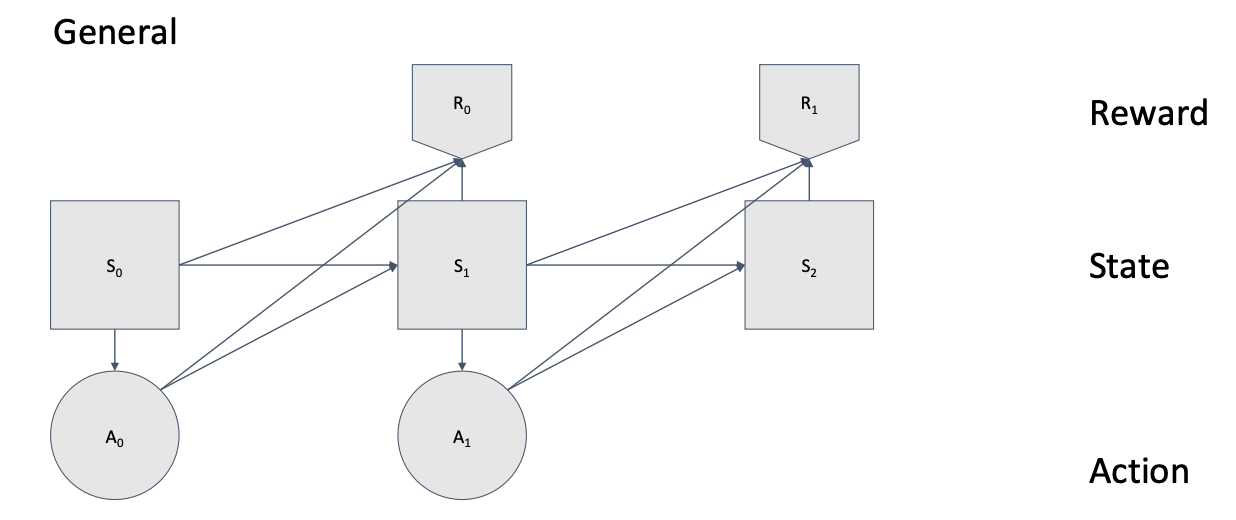
\includegraphics[width=\linewidth]{interaction_sequential.png}
\end{center}


\textit{Reinforcement Learning (RL)} \smallskip

RL is an interdisciplinary area of machine learning and optimal control concerned with how an intelligent agent ought to take actions in a dynamic environment to maximize the cumulative reward. 

\begin{center}
	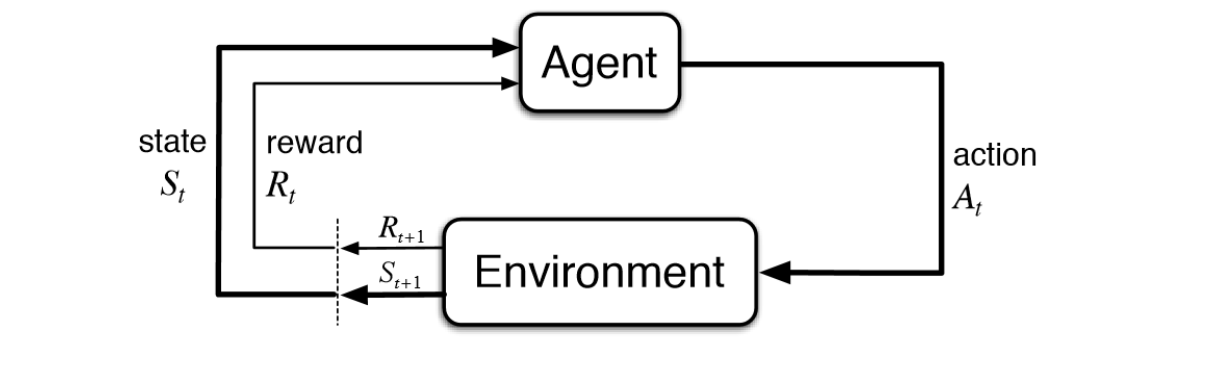
\includegraphics[width=\linewidth]{reinforcement_learning.png}
\end{center}

Example for state, action and rewards: 
\begin{center}
	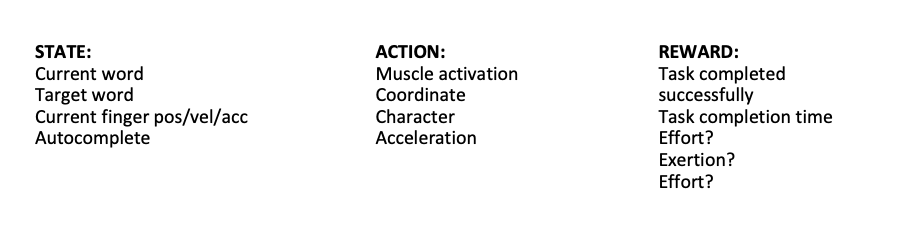
\includegraphics[width=\linewidth]{example_RL.png}
\end{center}

What is the optimal action to take given a state? \smallskip


\textit{Difference from RL to other ML paradigms} \smallskip

\begin{minipage}{\linewidth} 
	\centering
	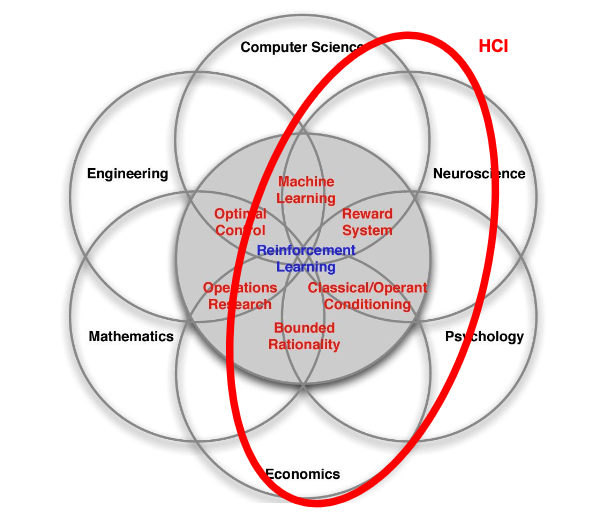
\includegraphics[width=0.45\linewidth]{HCI.png}
	\quad 
	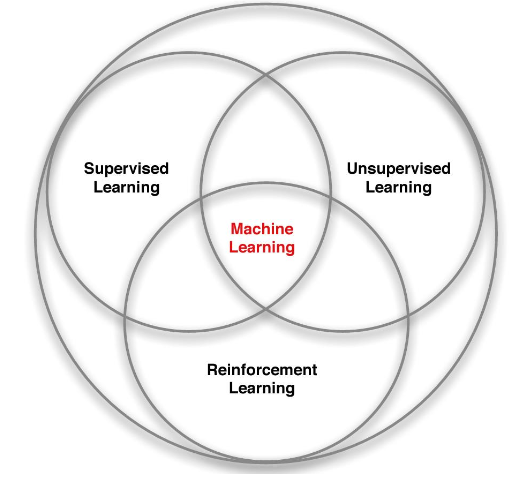
\includegraphics[width=0.45\linewidth]{machine_learning.png}
  \end{minipage}

\begin{itemize}[itemsep=-5pt, topsep=0pt, leftmargin=*]
	\item No supervisor, only a reward signal
	\item feedback is delayed, not instantaneous
	\item Time really matters (sequential, non i.i.d data)
	\item Agent's actions affect the subsequent data it receives
\end{itemize}

\textit{Markov Decision Process} \smallskip

Tuple: $\{S, A, T, R, \gamma\}$

\begin{itemize}[itemsep=-5pt, topsep=0pt, leftmargin=*]
	\item S: A finite set of states (what letters have I typed so far)
	\item A: A finite set of actions (what letter do I type next, what muscle do I activate)
	\item T: Transition matrix: $p(s', a, s)$ given state and action, what is the prob of the next state
	\item R: Reward $R(s', a, ss)$ the immediate reward of taking the action $a$ in state $s$. 
	\item $\gamma \in [0, 1)$: the discount factor
\end{itemize}


\textit{Optimal action given a state} \smallskip

Policy is the agent's bahavior. It maps a state to an action to maximize the cumulative reward. 

The goal is to find an optimal policy: $\pi$ \smallbreak

\textit{Value Function} \smallskip

Value function is a prediction of future reward. Used to evaluate the goodness/badness of states. Therefore select between actions. 

$$V_{\pi}(s) = E_{\pi}[R_{t+1} + \gamma R_{t+2} + \gamma^2 R_{t+3} + ... | s_{t} = s]$$

\textit{On Rewards} \smallskip
It is a scalar feedback and describes how well an agent is doing at step t. 


The reward hypothesis states that all goals can be described by the maximization of the expected cumulative reward. 

\textbf{Bounded Rationality}

Supposed to look at Human-likeness.

\textit{Comparison with Standard RL} \smallskip

\begin{center}
	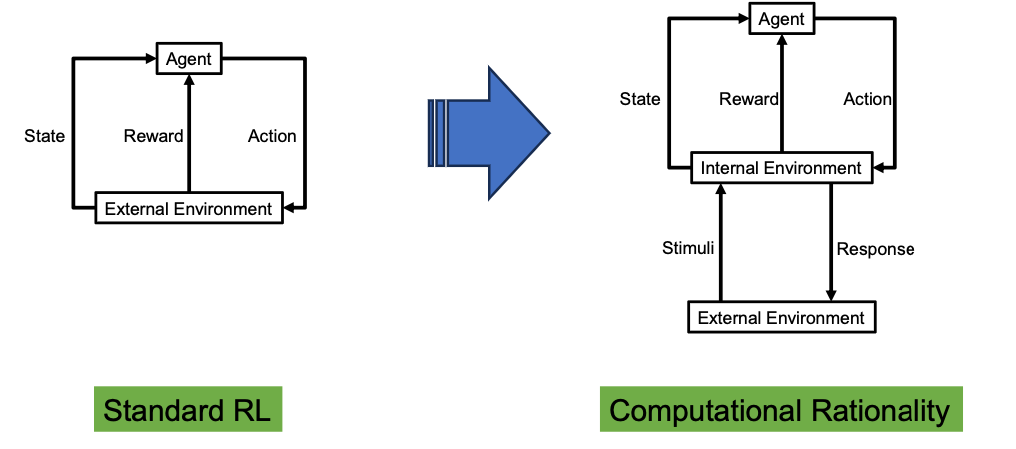
\includegraphics[width=\linewidth]{comparison_RL.png}
\end{center}

\textit{Internal vs External Environmen} \smallskip

\begin{itemize}[itemsep=-5pt, topsep=0pt, leftmargin=*]
	\item Humans acit in the external environment via their internal environment
	\item External environment: The world
	\item Internal environment: Cognition
	\item Agent: Decison maker
\end{itemize}

Interaction emerges as adaption within internal and external bounds. 


\begin{center}
	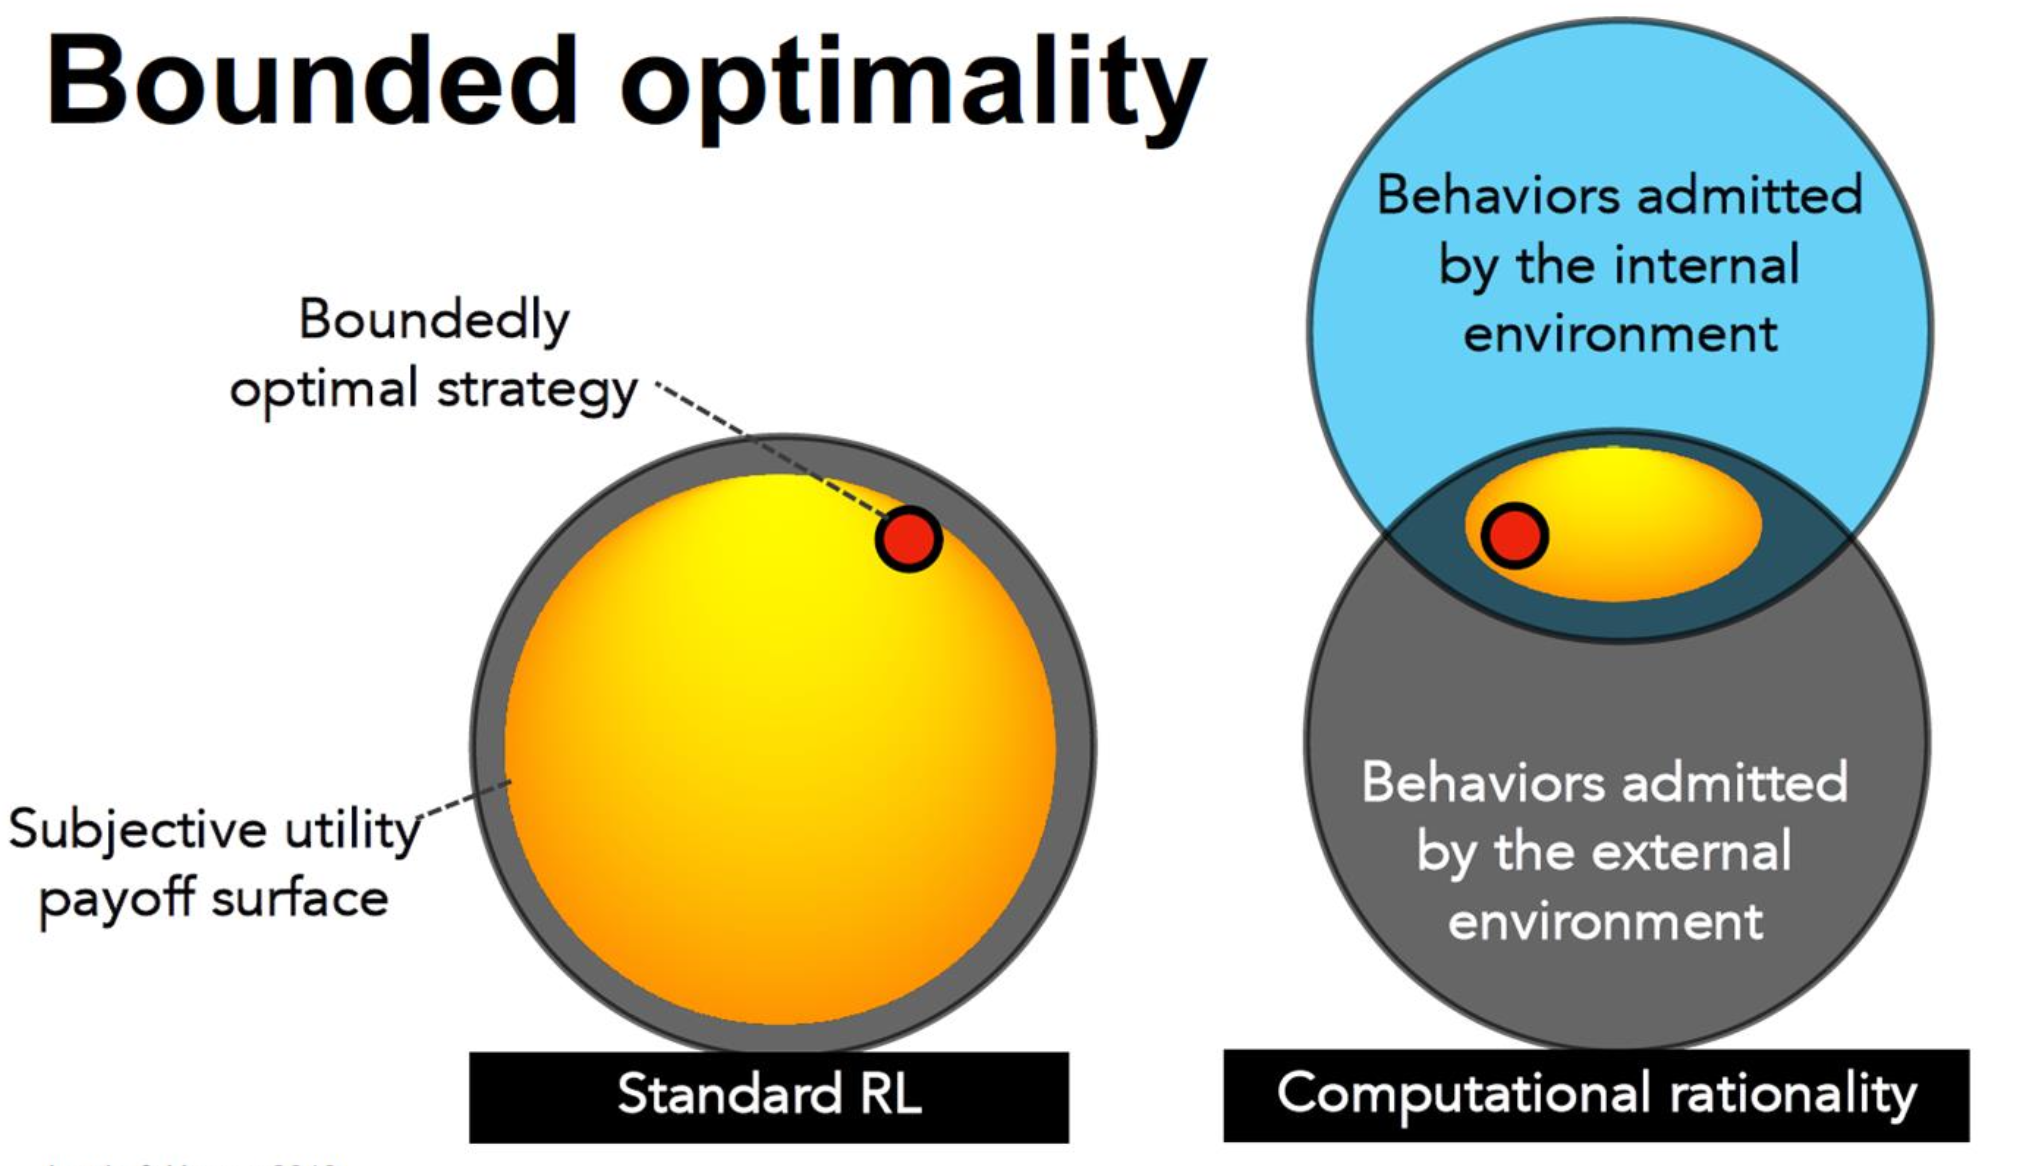
\includegraphics[width=\linewidth]{bounded_optimality.png}
\end{center}


\begin{center}
	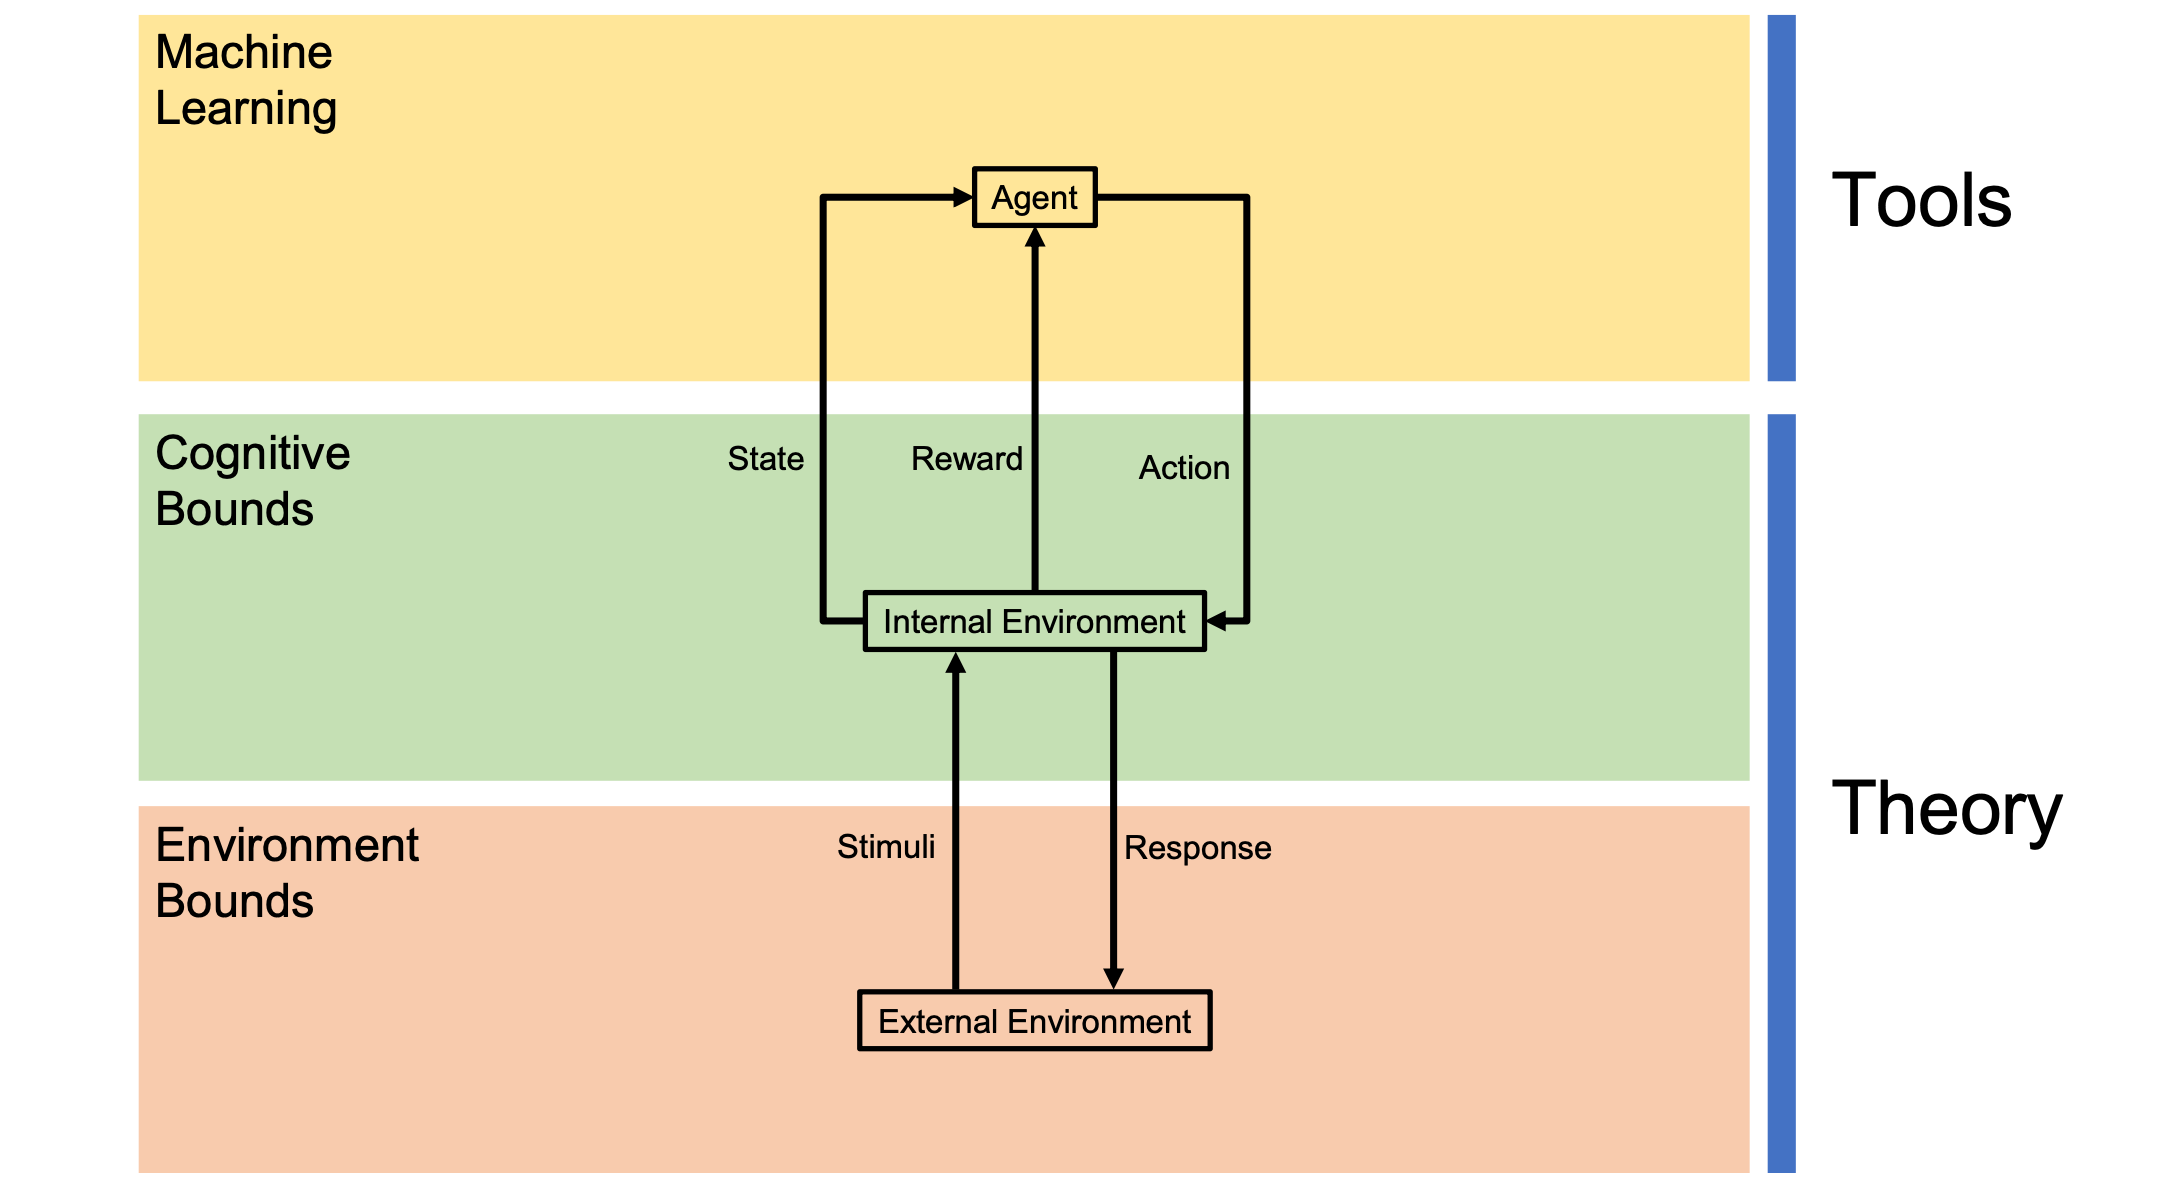
\includegraphics[width=\linewidth]{ml_and_bounds.png}
\end{center}




\begin{center}
	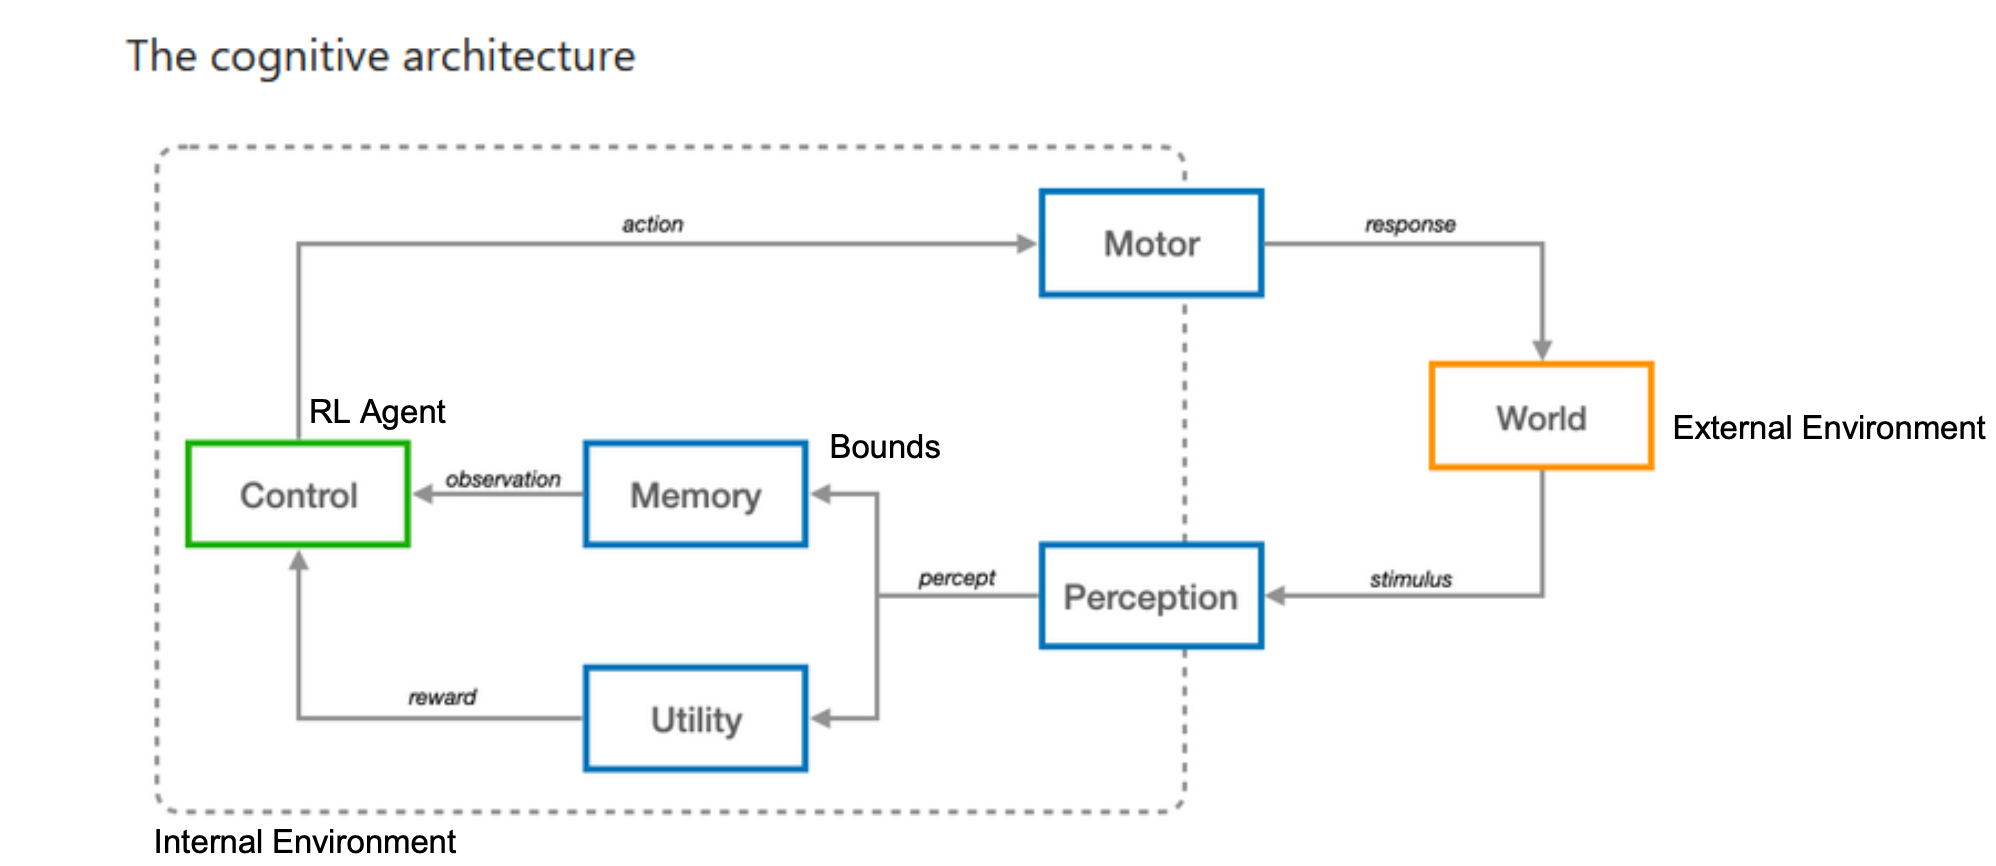
\includegraphics[width=\linewidth]{cognitive_architecture.png}
\end{center}


\textbf{Key cognitive capacities in HCI} \smallskip

\begin{itemize}[itemsep=-5pt, topsep=0pt, leftmargin=*]
	\item (Suvervisory Control): Adaptively deciding goals, allocating cognitive resources to tasks, and changing course of action when required. 
	\item Memory: Forming, maintaining and accessing beliefs about objects that are not directly perceivable
	\item Attention: Selectively processing some part of the perceptual failed
	\item Reasoning: Applying transformation rules to beliefs to form new beliefs
	\item Gathering information and choosing between options
\end{itemize}

\textit{General props of Human Cognition} \smallskip

\begin{itemize}[itemsep=-5pt, topsep=0pt, leftmargin=*]
	\item Goal-oriented
	\item Adapts
	\item Learns
	\item Carries out computations on representations
	\item Is limited
	\item Requires energy and effort
\end{itemize}


\textit{1. Cognition is goal oriented} \smallskip

How do we choose what stimuli to direct our cognitive resources on. We use cognitive control to decide to which goal we direct thinking and action.

\begin{itemize}[itemsep=-5pt, topsep=0pt, leftmargin=*]
	\item Setting goals
	\item Directing resources and Attention
	\item Multitasking
	\item Task-switching
	\item Inhibiting distracting ideas
\end{itemize}

\textit{2. Cognition Adapts} \smallskip

Systems used by people and the way work is carried out changes all the time. 
\begin{itemize}[itemsep=-5pt, topsep=0pt, leftmargin=*]
	\item Cognitive, motor and perceptual processes need to adapt constantly
	\item Update old beliefs with new ones
	\item Update old plans and form new ones
	\item Cognition is not only reacting to environments but also actively finding ways to function better
\end{itemize}


\textit{3. Cognition Learns} \smallskip

Computers are complex but opaque systems. We need internal representations to control them and need to have multiple memory systems to that end. 
It learns to use external aids. 

Cognition also learns how to use external aids such as notes calculators etc. to augment our abilities. This changes the way we use cognition in interaction. 
Example is GUIs that have lead to forget commands in memory. 


Example: Menu interaction of non-sighted users
\begin{center}
	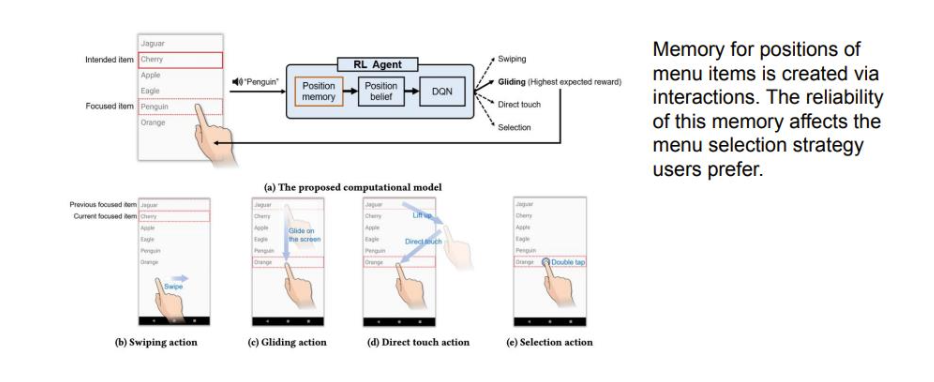
\includegraphics[width=\linewidth]{Cognition_learns_example.png}
\end{center}


\textit{4. Cognition computes based on internal representations} \smallskip

 Cognition can reason about things that are not directly perceivable. It uses internal models of reality to reason, formulate goals and plans.

 Examples are metaphors to help users understand an UI. Desktop metaphor uses spatial concepts that are rooted in everyday physical experiences. 

\textit{5. Cognition is limited \& costs energy} \smallskip

\begin{itemize}[itemsep=-5pt, topsep=0pt, leftmargin=*]
	\item Visual attention is spactially limited (periphery vs foveal region)
	\item Working memory is capacity-limited (only few mental representations active at a time, typically working memory is limited to 2-4 items)
	\item Forgetting occurs in long-term memory (we cannot remember everything we have experiences and thus forget details)
	\item Capacity for abstract reasoning and planning is limited (only think few steps ahead)
\end{itemize}


\textit{Perception} \smallskip

Perception is needed to regulate actions:
\begin{itemize}[itemsep=-5pt, topsep=0pt, leftmargin=*]
	\item UIs communicate their state via perception
	\item Visual, auditory and tactile perception each have own characteristics and roles in HCI
\end{itemize}

\begin{center}
	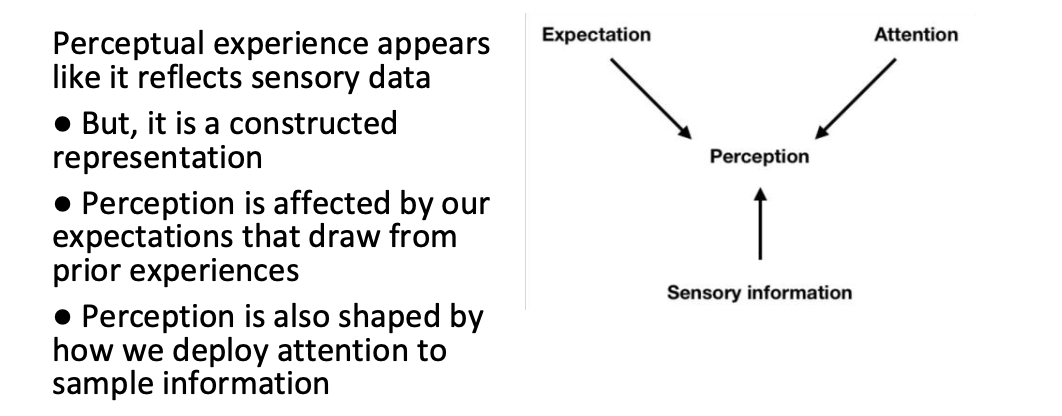
\includegraphics[width=\linewidth]{perception.png}
\end{center}


\textit{Elementary perceptual Tasks} \smallskip

\begin{itemize}[itemsep=-5pt, topsep=0pt, leftmargin=*]
	\item Discrimination: telling whether a difference occurs in sensory data
	\item Detection: telling whether an event of interest occurs or not
	\item Recognition: Categorizing a stimulus as something
	\item Estimation: estimate property of an object of event in the environment
	\item Search: localizing an object of interest
\end{itemize}

\textbf{Gaze-based Interaction} \smallskip

Proble of selecting items on a computer with eye movements and fixations. These eyemovements obey Fitt's Law. 
Movement time of the eyes is proportional to distance and inversely proportional to size of the target.


\begin{center}
	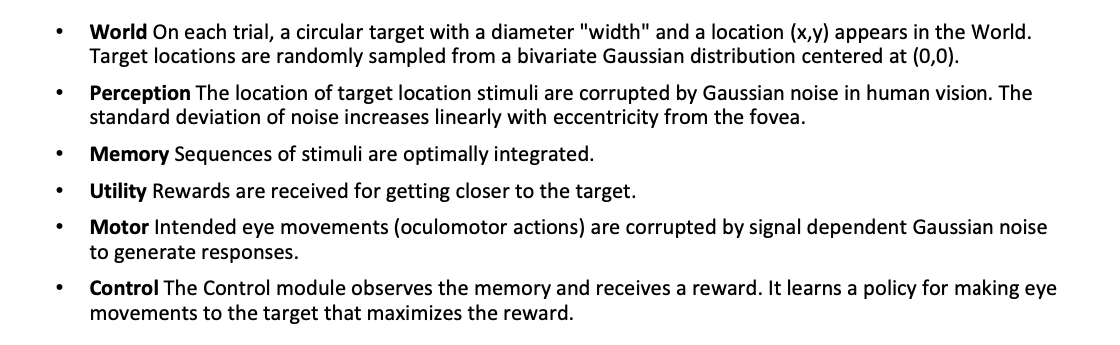
\includegraphics[width=\linewidth]{Gaze_based_interaction.png}
\end{center}



\textit{Comparison with Cognitive Architectures}


\begin{center}
	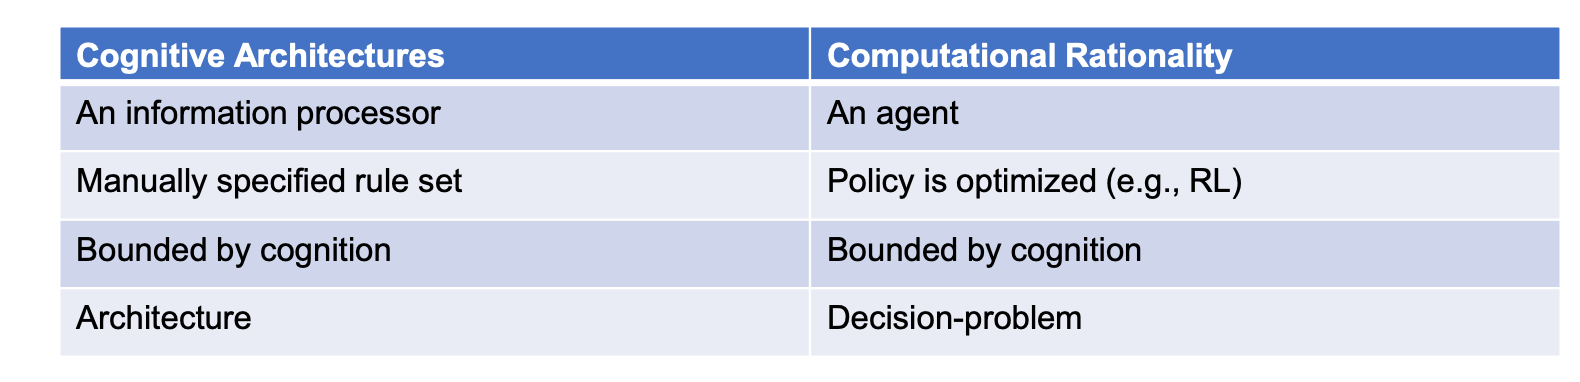
\includegraphics[width=\linewidth]{comparison_cognitive_architectures.png}
\end{center}












